\documentclass[aspectratio=43]{beamer}

% Title --------------------------------------------
\title{\huge Course wrap-up}
\author{Francisco Villamil}
\date{War, peace, and political violence\\UC3M, Fall 2024}

%%% NOTE -- CHECK THIS: https://github.com/paulgp/beamer-tips


%%% Building heavily on https://github.com/kylebutts/templates

% xcolor, define them
\usepackage{xcolor}

% TEXT COLORS
\definecolor{red}{HTML}{9a2515}
\definecolor{yellow}{HTML}{EBC944}
\definecolor{asher}{HTML}{555F61}
\definecolor{jet}{HTML}{131516}

% THEME COLORS
\definecolor{accent}{HTML}{107895}
\definecolor{accent2}{HTML}{9a2515}

% Color commands
\newcommand\red[1]{{\color{red}#1}}
\newcommand\yellow[1]{{\color{yellow}#1}}
\newcommand\asher[1]{{\color{asher}#1}}

\newcommand\BGred[1]{{\colorbox{red!80!white}{#1}}}
\newcommand\BGyellow[1]{{\colorbox{yellow!80!white}{#1}}}
\newcommand\BGasher[1]{{\colorbox{asher!80!white}{#1}}}

\renewcommand<>{\BGyellow}[1]{\only#2{\beameroriginal{\BGyellow}}{#1}}

% Appendix numbering
\usepackage{appendixnumberbeamer}

% Beamer Options -------------------------------------

% Background
\setbeamercolor{background canvas}{bg = white}

% Change text margins
\setbeamersize{text margin left = 25pt, text margin right = 15pt}

% \alert
\setbeamercolor{alerted text}{fg = accent2}

% Frame title
\setbeamercolor{frametitle}{bg = white, fg = jet}
\setbeamercolor{framesubtitle}{bg = white, fg = accent}
\setbeamerfont{framesubtitle}{size = \small, shape = \itshape}

% Block
\setbeamercolor{block title}{fg = white, bg = accent2}
\setbeamercolor{block body}{fg = jet, bg = jet!10!white}

% Title page
\setbeamercolor{title}{fg = jet}
\setbeamercolor{subtitle}{fg = accent}

%% Custom \maketitle and \titlepage
\setbeamertemplate{title page}
{
    \begin{centering}
      % \vspace{20mm}
      {\Large \usebeamerfont{title}\usebeamercolor[fg]{title}\inserttitle}\\ \vskip0.25em%
      \ifx\insertsubtitle\@empty%
      \else%
        {\usebeamerfont{subtitle}\usebeamercolor[fg]{subtitle}\insertsubtitle\par}%
      \fi%
      {\vspace{10mm}\insertauthor}\\
      \ifx\insertinstitute\@empty%
      \else%
        {\vspace{5mm}\color{asher}\scriptsize{\insertinstitute}}
      \fi%
      {\color{asher}\small{\insertdate}}\\
    \end{centering}
}

% Table of Contents
\setbeamercolor{section in toc}{fg = accent!70!jet}
\setbeamercolor{subsection in toc}{fg = jet}

% Button
\setbeamercolor{button}{bg = accent}

% Remove navigation symbols
\setbeamertemplate{navigation symbols}{}

% Table and Figure captions
\setbeamercolor{caption}{fg=jet!70!white}
\setbeamercolor{caption name}{fg=jet}
\setbeamerfont{caption name}{shape = \itshape}

% Put slide number / total slides at the bottom right
\makeatother
\makeatletter
\setbeamertemplate{footline} %{\hfill\insertframenumber/\inserttotalframenumber}
{%
  \leavevmode%
  \hbox{
  \begin{beamercolorbox}[wd=\paperwidth,ht=2.5ex,dp=1.125ex,leftskip=.3cm,rightskip=.3cm plus1fil]{footlinecolor}%
    \color{asher}{\hfill\insertframenumber/\inserttotalframenumber}
  \end{beamercolorbox}}%
  \vskip0pt%
}
\makeatother
\makeatletter

% Bullet points

%% Fix left-margins
\settowidth{\leftmargini}{\usebeamertemplate{itemize item}}
\addtolength{\leftmargini}{\labelsep}

%% enumerate item color
\setbeamercolor{enumerate item}{fg = accent}
\setbeamerfont{enumerate item}{size = \small}
\setbeamertemplate{enumerate item}{\insertenumlabel.}

%% itemize
\setbeamercolor{itemize item}{fg = accent!70!white}
\setbeamerfont{itemize item}{size = \small}
\setbeamertemplate{itemize item}[circle]
\setlength{\itemsep}{0pt plus 6pt}

%% right arrow for subitems
\setbeamercolor{itemize subitem}{fg = accent!60!white}
\setbeamerfont{itemize subitem}{size = \small}
\setbeamertemplate{itemize subitem}{$\rightarrow$}

\setbeamertemplate{itemize subsubitem}[square]
\setbeamercolor{itemize subsubitem}{fg = jet}
\setbeamerfont{itemize subsubitem}{size = \small}

% References

%% Bibliography Font, roughly matching aea
\setbeamerfont{bibliography item}{size = \footnotesize}
\setbeamerfont{bibliography entry author}{size = \footnotesize, series = \bfseries}
\setbeamerfont{bibliography entry title}{size = \footnotesize}
\setbeamerfont{bibliography entry location}{size = \footnotesize, shape = \itshape}
\setbeamerfont{bibliography entry note}{size = \footnotesize}

\setbeamercolor{bibliography item}{fg = jet}
\setbeamercolor{bibliography entry author}{fg = accent!60!jet}
\setbeamercolor{bibliography entry title}{fg = jet}
\setbeamercolor{bibliography entry location}{fg = jet}
\setbeamercolor{bibliography entry note}{fg = jet}

%% Remove bibliography symbol in slides
\setbeamertemplate{bibliography item}{}





% Links ----------------------------------------------

\usepackage{hyperref}
\hypersetup{
  colorlinks = true,
  linkcolor = accent,
  filecolor = accent,
  urlcolor = accent,
  citecolor = accent,
}


% Line spacing --------------------------------------
\usepackage{setspace}
\setstretch{1.2}


% \begin{columns} -----------------------------------
\usepackage{multicol}


% % Fonts ---------------------------------------------
% % Beamer Option to use custom fonts
% \usefonttheme{professionalfonts}
%
% % \usepackage[utopia, smallerops, varg]{newtxmath}
% % \usepackage{utopia}
% \usepackage[sfdefault,light]{roboto}
%
% % Small adjustments to text kerning
% \usepackage{microtype}



% Remove annoying over-full box warnings -----------
\vfuzz2pt
\hfuzz2pt


% Table of Contents with Sections
\setbeamerfont{myTOC}{series=\bfseries, size=\Large}
\AtBeginSection[]{
        \frame{
            \frametitle{Roadmap}
            \tableofcontents[current]
        }
    }


% References ----------------------------------------
\usepackage[
    citestyle= authoryear,
    style = authoryear,
    natbib = true,
    backend = biber
]{biblatex}

% Smaller font-size for references
\renewcommand*{\bibfont}{\small}

% Remove "In:"
\renewbibmacro{in:}{}

% Color citations for slides
\newenvironment{citecolor}
    {\footnotesize\begin{color}{accent2}}
    {\end{color}}

\newcommand{\citetcolor}[1]{{\footnotesize\textcolor{asher}{\citet{#1}}}}
\newcommand{\citepcolor}[1]{{\footnotesize\textcolor{asher}{\citep{#1}}}}

% Tables -------------------------------------------
% Tables too big
% \begin{adjustbox}{width = 1.2\textwidth, center}
\usepackage{adjustbox}
\usepackage{array}
\usepackage{threeparttable, booktabs, adjustbox}

% Fix \input with tables
% \input fails when \\ is at end of external .tex file

\makeatletter
\let\input\@@input
\makeatother

% Tables too narrow
% \begin{tabularx}{\linewidth}{cols}
% col-types: X - center, L - left, R -right
% Relative scale: >{\hsize=.8\hsize}X/L/R
\usepackage{tabularx}
\newcolumntype{L}{>{\raggedright\arraybackslash}X}
\newcolumntype{R}{>{\raggedleft\arraybackslash}X}
\newcolumntype{C}{>{\centering\arraybackslash}X}

% Figures

% \imageframe{img_name} -----------------------------
% from https://github.com/mattjetwell/cousteau
\newcommand{\imageframe}[1]{%
    \begin{frame}[plain]
        \begin{tikzpicture}[remember picture, overlay]
            \node[at = (current page.center), xshift = 0cm] (cover) {%
                \includegraphics[keepaspectratio, width=\paperwidth, height=\paperheight]{#1}
            };
        \end{tikzpicture}
    \end{frame}%
}

% subfigures
\usepackage{subfigure}


% Highlight slide -----------------------------------
% \begin{transitionframe} Text \end{transitionframe}
% from paulgp's beamer tips
\newenvironment{transitionframe}{
    \setbeamercolor{background canvas}{bg=accent!60!black}
    \begin{frame}\color{accent!10!white}\LARGE\centering
}{
    \end{frame}
}


% Table Highlighting --------------------------------
% Create top-left and bottom-right markets in tabular cells with a unique matching id and these commands will outline those cells
\usepackage[beamer,customcolors]{hf-tikz}
\usetikzlibrary{calc}
\usetikzlibrary{fit,shapes.misc}

% To set the hypothesis highlighting boxes red.
\newcommand\marktopleft[1]{%
    \tikz[overlay,remember picture]
        \node (marker-#1-a) at (0,1.5ex) {};%
}
\newcommand\markbottomright[1]{%
    \tikz[overlay,remember picture]
        \node (marker-#1-b) at (0,0) {};%
    \tikz[accent!80!jet, ultra thick, overlay, remember picture, inner sep=4pt]
        \node[draw, rectangle, fit=(marker-#1-a.center) (marker-#1-b.center)] {};%
}



\begin{document}

\begin{frame}
  \titlepage
\end{frame}

% ----------------------------------------------------
\begin{frame}
\frametitle{Overview}
\centering

\begin{itemize}
  \item[1.] Wars at the international level
  \item<2->[2.] Internal conflict
  \item<3->[3.] What happens \textit{within} conflicts
  \item<4->[4.] What happens \textit{after} conflicts
  \item<5->[]
  \item<5->[$\rightarrow$] Putting it all together
\end{itemize}

\end{frame}
% ----------------------------------------------------

% ----------------------------------------------------
\begin{frame}
\frametitle{Overview}
\centering

\begin{tabular}{m{1.75cm}|m{4cm}m{4cm}}
& {\color{gray}{\footnotesize Target:}} \newline State & {\color{gray}{\footnotesize Target:}} \newline Non-State \\\hline\\
{\color{gray}{\footnotesize Perpetrator:}} \newline State & Interstate war & State repression \newline Genocide \newline Ethnic cleansing \\\\
{\color{gray}{\footnotesize Perpetrator:}} \newline Non-State & Organized crime \newline Mass protests (rebellion) \newline Military coup \newline Political assassination* \newline Civil War \newline Terrorism & Intercommunal violence\\\\\hline
\end{tabular}

\end{frame}
% ----------------------------------------------------

% ----------------------------------------------------
\begin{frame}
\frametitle{Connecting logics}
\centering

\begin{itemize}
  \item \BGyellow<1>{Hierarchy}
  \begin{itemize}
    \item civil wars engender genocide, or violence against civilians
  \end{itemize}
  \item<2-> \BGyellow<2>{Instrumentalization}
  \begin{itemize}
    \item intercommunal violence used as a method for genocide, terrorism employed as part of wars...
  \end{itemize}
  \item<3-> \BGyellow<3>{Escalation}
  \begin{itemize}
    \item civil wars and international wars, Arab Spring, ...
  \end{itemize}
  \item<4-> \BGyellow<4>{Substitution}
  \begin{itemize}
    \item proxy wars (Cold War), coup-proofing via purging, terrorism ...
  \end{itemize}
\end{itemize}

\end{frame}
% ----------------------------------------------------

% ----------------------------------------------------
\imageframe{img/syria1}
% ----------------------------------------------------

% ----------------------------------------------------
\imageframe{img/syria2}
% ----------------------------------------------------

% ----------------------------------------------------
\imageframe{img/syria3}
% ----------------------------------------------------

% ----------------------------------------------------
\imageframe{img/syria4}
% ----------------------------------------------------

% ----------------------------------------------------
\imageframe{img/syria5}
% ----------------------------------------------------

% ----------------------------------------------------
\imageframe{img/syria6}
% ----------------------------------------------------

% ----------------------------------------------------
\begin{frame}[plain]
  \begin{tikzpicture}[remember picture, overlay]
      \node[at = (current page.center), yshift = 2cm] (cover) {%
          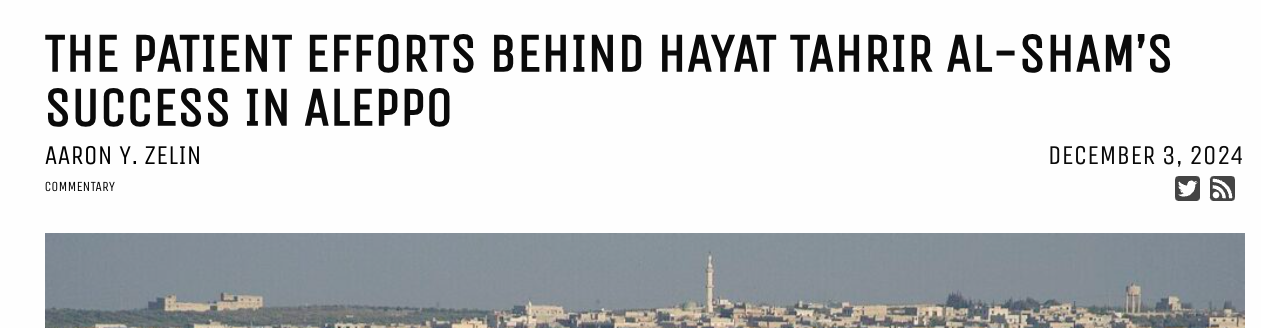
\includegraphics[keepaspectratio, width=\paperwidth]{img/syria7a}};
      \node[at = (current page.center), yshift = -2cm] (cover) {%
          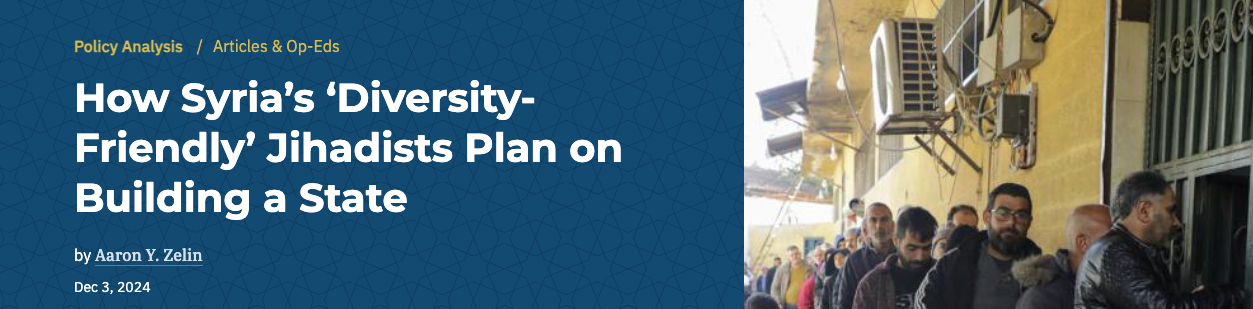
\includegraphics[keepaspectratio, width=\paperwidth]{img/syria7b}};
  \end{tikzpicture}
\end{frame}%
% ----------------------------------------------------

% ----------------------------------------------------
\imageframe{img/syria8}
% ----------------------------------------------------

% ----------------------------------------------------
\imageframe{img/syria9}
% ----------------------------------------------------

% ----------------------------------------------------
\imageframe{img/syria10}
% ----------------------------------------------------

% ----------------------------------------------------
\imageframe{img/syria11}
% ----------------------------------------------------

% ----------------------------------------------------
\begin{frame}
\frametitle{Issues in Syrian civil war}
\centering

\begin{itemize}
  \item Link between non-violence and war
  \item Role of state repression
  \item Rebel group fragmentation and alliances
  \item Rebel governance
  \item Postwar power-sharing
  \item Internationalized civil wars
  \item (...)
\end{itemize}

\end{frame}
% ----------------------------------------------------
  

% ----------------------------------------------------
\begin{frame}
\frametitle{Final exam}
\centering

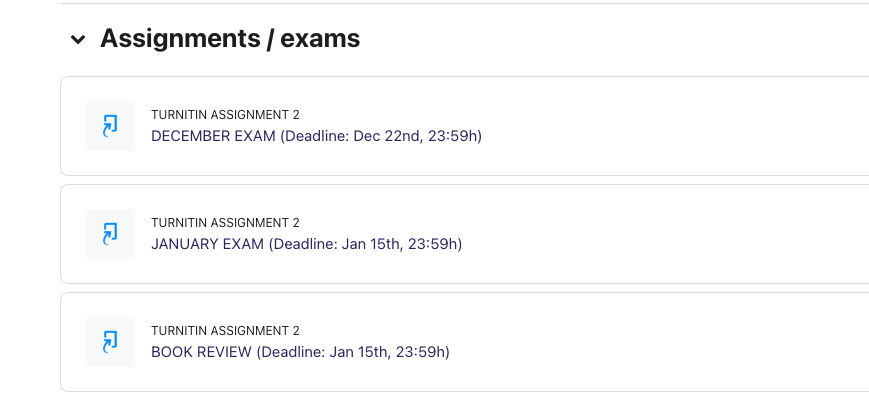
\includegraphics[width = \textwidth]{img/ag}

Submission in Aula Global (\textbf{send a PDF})

\end{frame}
% ----------------------------------------------------

% ----------------------------------------------------
\begin{frame}
\frametitle{\textbf{Book review}}
\centering

\begin{itemize}
  \item Main idea: link what's in the book to some theory or ideas about political violence we've covered
  \item \textbf{Not} a summary of the book
  \begin{itemize}
    \item Critique probably doesn't work either: many of these are journalistic books that tell what happened, not why or how (exceptions)
  \end{itemize}
  \item Can cover one issue in depth or many more superficially
  \item \textbf{Word limit}: 2500 words (no formal minimum, but ca. 1000 words)
  \item Deadline is January 15 but can submit anytime
\end{itemize}

\end{frame}
% ----------------------------------------------------


% ----------------------------------------------------
\begin{frame}
\frametitle{\textbf{Take-home essay}}
\centering

\begin{itemize}
  \item Two questions, 4 \& 2 points each, 1000/500 words max
  \item I'll send the exam the previous evening
\end{itemize}

\end{frame}
% ----------------------------------------------------

% ----------------------------------------------------
\begin{frame}
\frametitle{Take-home essay, short Q examples}
\centering

\begin{itemize}
  \item[\textbf{Q1:}] (2 points, 500 words) Last January 6th, the US Capitol was stormed by a crowd of Trump supporters. Can we consider that event as an instance of political violence? Why or why not? Can we consider it as an example of a coup d'état attempt? Why or why not?
\end{itemize}

\end{frame}
% ----------------------------------------------------

% ----------------------------------------------------
\begin{frame}
\frametitle{Take-home essay, short Q examples}
\centering

\begin{itemize}
  \item[\textbf{Q1:}] (2 points, 500 words) Last year, Israel designated six Palestinian organizations who carry out NGO work as terrorist organizations (see this news article in \textit{Haaretz}: \url{https://bit.ly/3GGCVeu}). The Israeli government claimed that, although these are NGOs, they ``are controlled by the senior leadership of the PFLP and employ many members of the group ... including activists who were involved in terrorism.'' [The PFLP, or Popular Front for the Liberation of Palestine, is an armed organization that has been long designated as a terrorist organization by both the US and European Union, among other countries.] Do you agree with the Israeli decision? Why or why not?
\end{itemize}

\end{frame}
% ----------------------------------------------------

% ----------------------------------------------------
\begin{frame}
\frametitle{Take-home essay, long Q examples}
\centering

\begin{itemize}
  \item[\textbf{Q2:}] (4 points, 1000 words) Brexit, and the Northern Ireland Protocol in particular, has brought tensions to Northern Ireland. In Spring 2021 there were loyalist protests that eventually evolved into ethnic riots. Some voices now warn of the risk of larger scale political violence returning to the region. What do you think are the risk factors and/or what could be done to avoid another conflict? What is it different now than when the Troubles started in the late 1960s?
\end{itemize}

\end{frame}
% ----------------------------------------------------

% ----------------------------------------------------
\begin{frame}
\frametitle{Take-home essay, long Q examples}
\centering

\begin{itemize}\small
  \item[\textbf{Q2:}] (4 points, 1000 words) Protests have recently erupted in Kazakhstan and quickly escalated into violence between protesters and state forces, including Russian forces sent in by Putin, leaving more than 150 deaths, before calm returned earlier this week. What was the actual risk of large-scale violence in Kazakhstan? Should we be surprised that the protests did not escalate into e.g. a civil war? Is there risk of conflict in the short- to medium-term, like in other Central Asian countries?
\end{itemize}

\setstretch{0.9}

\begin{itemize}
  \item ({\footnotesize There are many factors related to the escalation and onset of violence: structural conditions (economy, geography, ...), political relations (government/opposition dynamics, previous history of violence, ...), international politics, etc. You can focus on one of these factors or on many, and you can discuss risk factors, restraint factors (why a war is unlikely), or both. For background in Central Asia, you can check  \href{https://ucdp.uu.se/}{UCDP Encyclopedia}, \href{https://growup.ethz.ch/atlas/}{EPR ethnic data}, Wikipedia, newspapers, etc.})
\end{itemize}

\end{frame}
% ----------------------------------------------------

% ----------------------------------------------------
\imageframe{img/chatgpt}
% ----------------------------------------------------
  

\end{document}
